\documentclass{article}
\usepackage{graphicx}
\graphicspath{ {./} }

\author{Zixiang Wang, Suyash Thapa}
\title{Project Documentation}


\begin{document}

\maketitle

\section{ER Diagram}
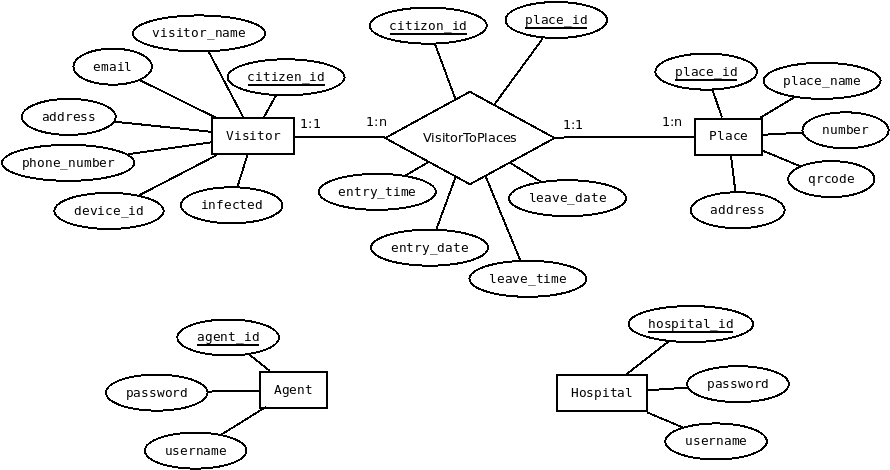
\includegraphics[scale=0.5]{./er-diagram.png}

\section{Page Design}

\subsection*{Page Structure}

%display the diagram
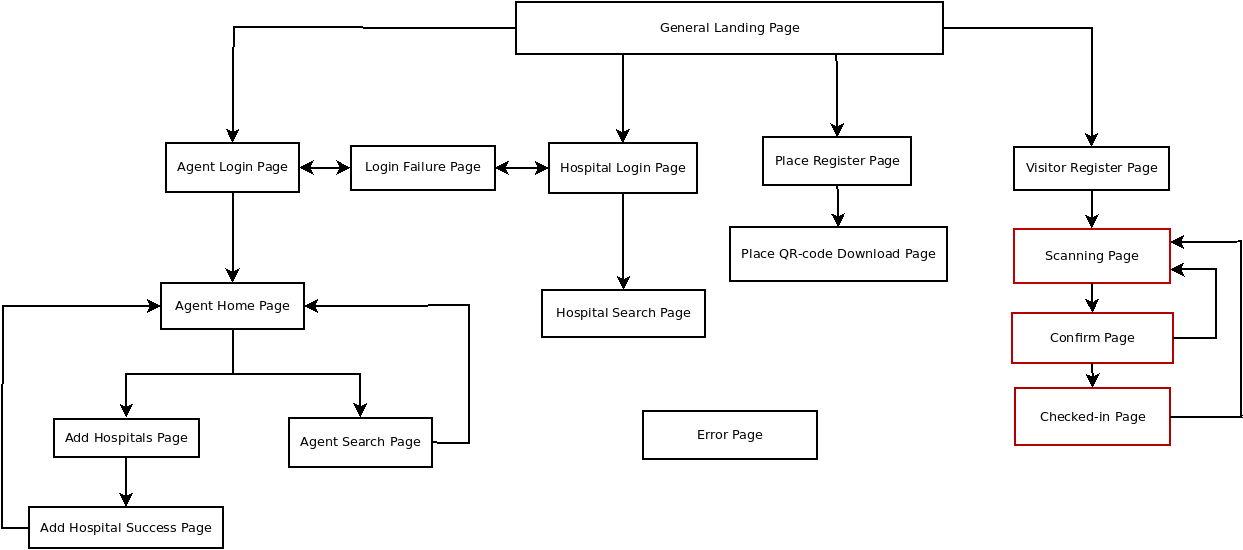
\includegraphics[scale=0.35]{./pages-structure.png}
Pages that marked red cannot returns to the general landing page via navbar.

\subsection*{Page Descriptions}
\subsubsection*{General Pages \& Components}
Navbar
\begin{itemize}
	\item contains a logo of the website on the most left.
  	\item contains links which differs in different pages on the left side.
  	\item contains link to imprint.
  	\item a log out button should show on the right side after agent or hospital login.
  	\item every page contains a navbar.
  	\item when not logged in when clicking the logo it directs to the general landing page.
	\item when logged in as agent clicking the logo directs to agent main page.
	\item when logged in as hospital clicking the logo directs to itself.
\end{itemize}
\\ 
\\ 
\textbf{1. General Landing Page}\\
Components:
\begin{itemize}
	\item Navbar
\end{itemize}
The Navbar should contains:
\begin{itemize}
	\item logo
	\item link to visitor registration page
	\item link to agency login page
	\item link to hospital login page
	\item link to place register page
	\item link to imprint
\end{itemize}
\\
\textbf{2. Error Page}\\
Error page is shown when error occurs. It shows to user that something goes wrong.\\
Components:
\begin{itemize}
	\item Navbar
\end{itemize}
The Navbar should contains:
\begin{itemize}
	\item logo (links to the general landing page)
	\item link to visitor registration page
	\item link to agency login page
	\item link to hospital login page
	\item link to place register page
	\item link to imprint
\end{itemize}


\subsubsection*{Agents' Story}
\textbf{3. Agent Login Page}\\
Agent login page provide interface to let agents login their account.\\
When clicking the logo in the navbar, it directs to the general landing page.
Components:
\begin{itemize}
	\item Navbar
	\item a form takes two inputs: username, password
	\item a login button to submit username and password inputed by agent
\end{itemize}
The Navbar should contains:
\begin{itemize}
	\item logo (links to general landing page)
	\item link to imprint
	\item a logout button on the right
\end{itemize}
\\
\textbf{4. Agent Home Page}\\
Agent home page directs agent to either add hospital page or search page.\\
Components:
\begin{itemize}
	\item Navbar
	\item a button link to add hospital page
	\item a button link to agent search page
\end{itemize}
The Navbar should contains:
\begin{itemize}
	\item logo (links to itself)
	\item link to imprint
	\item a logout button on the right
\end{itemize}
\\
\textbf{5. Add Hospital Page}\\
Add hospital page allows agents to add a hospital with its hospital\_id, username, password.\\
Components:
\begin{itemize}
	\item Navbar
	\item a form that takes three inputs: hospital\_id, username, password
	\item a button link to add hospital page
	\item a button link to agent search page
\end{itemize}
The Navbar should contains:
\begin{itemize}
	\item logo (links to agent home page)
	\item link to imprint
	\item a logout button on the right
\end{itemize}
\\
\textbf{6. Add Hospital Success Page}\\
Inform agents that the adding of hospital is succeeded.\\
Components:
\begin{itemize}
	\item Navbar
	\item text shows that the adding is succeeded.
\end{itemize}
The Navbar should contains:
\begin{itemize}
	\item logo (links to agent home page)
	\item link to imprint
	\item a logout button on the right
\end{itemize}
\\
\textbf{7. Agent Search Page}\\
Allow agents to search by place and/or person. Allow agents to modify all the data.\\
Components:\\
\textbf{1.} List places a person have been in a given time.\\
This section takes visitor's name, entry-time, entry-date, leave-time, leave-date as input.\\
And the result should be a table with five columns which are place name, entry-time, entry-date, 
leave-time, leave-date.\\
\textbf{2.} List visitors in a place with given time interval.\\
This section takes place name, entry-time, entry-date, leave-time, leave-date as input.\\
And the result should be a table with five columns: visitor's name, entry-time, entry-date, 
leave-date,\\
\textbf{3.} List visits (time interval the person spend in a given place) of a person in a particular place.\\
This section takes visitor's name and place name as input.\\
The result should be a table with five columns: visitor's name, entry-time, entry-date, leave-time, leave-date.\\
\textbf{4.} List with whom a particular person was at a particular place.\\
This section takes visitor's name and place name as input.\\
And the result should be a table with five columns: visitor's name, entry-time, entry-date, leave-time, leave-date.\\
\textbf{5.} Navbar\\
The Navbar should contains:
\begin{itemize}
	\item logo (links to agent home page)
	\item link to imprint
	\item a logout button on the right
\end{itemize}


\subsubsection*{Hospital's Story}
\textbf{8. Hospital Login Page}\\
Hospital login page allows hospital user to login.\\
Components:\\
\begin{itemize}
	\item Navbar
	\item a form takes three inputs: hospital\_id, username, password
	\item a login button to submit hospita\_id, username and password inputed by hospital user
\end{itemize}
Navbar
The Navbar should contains:
\begin{itemize}
	\item logo (links to general landing page)
	\item link to imprint
\end{itemize}

\textbf{9. Hospital Search Page (named hospital portal)}\\
This page allows hospital user to search a person by name and mark or unmark him/her as infected.
Components:\\
\begin{itemize}
	\item Navbar
	\item a form takes three inputs: hospital\_id, username, password
	\item a login button to submit hospita\_id, username and password inputed by hospital user
\end{itemize}
Navbar
The Navbar should contains:
\begin{itemize}
	\item logo (links to itself)
	\item link to imprint
\end{itemize}

\subsubsection*{Place Owner's Story}
\textbf{10. Place Register Page}\\
This page allows place owners to input information about their place and submit.
Components:\\
\begin{itemize}
	\item Navbar
	\item a form takes three inputs: place name, phone number, address
	\item a login button to submit place name, phone number, and address inputed by place owners
\end{itemize}
Navbar
The Navbar should contains:
\begin{itemize}
	\item logo (links to hospital home page)
	\item link to imprint
\end{itemize}

\textbf{11. Place QR-code Download Page}\\
This page contains QR-code, and by clicking on the QR-code, place owners can download the QR-code.
Components:\\
\begin{itemize}
	\item Navbar
	\item QR-code (by clicking on it, people can download the QR-code)
\end{itemize}
Navbar
The Navbar should contains:
\begin{itemize}
	\item logo (links to general landing page)
	\item link to imprint
\end{itemize}

\subsubsection*{Visitors' Story}
\textbf{12. Visitor Register Page}\\
This page allows visitors to register with their name, email, address, phone\_number, device\_id.
Once the visitors submit the informations, device\_id will be captured with consent of visitors, and 
visitors' infected attribute will be automatically marked 0 as default.
Components:\\
\begin{itemize}
	\item Navbar
	\item a form takes four inputs: name, email, address, phone\_number
	\item a login button to submit the form
\end{itemize}
Navbar
The Navbar should contains:
\begin{itemize}
	\item logo (links to general landing page)
	\item link to imprint
\end{itemize}

\textbf{13. Scanning Page}\\
This page let visitor scan the QR-code where they visit.
Components:\\
\begin{itemize}
	\item Navbar
	\item a camera section shows what the camera shot and can scan when detected a QR-code
\end{itemize}
Navbar
The Navbar should contains:
\begin{itemize}
	\item logo (links to itself)
	\item link to imprint
\end{itemize}

\textbf{14. Confirm Page}\\
This page let visitor to check whether the information they scanned correspond with the place they actual visit.
And confirm that they enter the place by clicking confirm button or cancel to enter the place.
Components:\\
\begin{itemize}
	\item Navbar
	\item a camera section shows what the camera shot and can scan when detected a QR-code
\end{itemize}
Navbar
The Navbar should contains:
\begin{itemize}
	\item logo (links to itself)
	\item link to imprint
\end{itemize}

\textbf{15. Checked-in Page}\\
This page shows the name of the place visitor entered, and for how long time the visitor stayed in the place.
And the visitor can check out the place by clicking a leave button. After visitor clicked the leave button, 
the page directs back to the scanning page, and submit visitor id, place id, entry time, entry date, leave time,
leave date to the back-end and save the visitor's visit.
Components:\\
\begin{itemize}
	\item Navbar
	\item a timer that shows for how long time the visitor stayed in the place
	\item a leave button to click when a visitor leave a place
\end{itemize}
Navbar
The Navbar should contains:
\begin{itemize}
	\item logo (links to itself)
	\item link to imprint
\end{itemize}


\end{document}
